\section{The Model}
As mentioned in the introduction, we will be simulating an \(N\)-Body problem including a heavy  object functioning as a star placed in the center of the system. The model will only cover the two-dimensional model.
The Model uses the LeapFrog integration method to approximate the new movements. 
Before we can apply Newton's equation however, we have to define our system of measurement and scale the corresponding physical constants.
Table \ref{tab:eenheden} displays the chosen Units for the corresponding physical quantity.

\begin{table}[h!]
\centering
\caption{The chosen Units of measurement}
\label{tab:eenheden}
\begin{tabular}{l|l|l}
  Physical quantity & Unit & SI-value \\ \hline
Time & 1 Month & \(2.629\cdot 10^{6}\) seconds  \\ 
 Distance & 1 Astronomical Unit (AU) & \(1.496\cdot10^{11}\) meters   \\
 Mass & 1 Earth Mass (\(M_\oplus\))& \(5.972\cdot10^{24}\) kilograms \\
\end{tabular}
\end{table}
Other units such as velocity, acceleration and density follow from these definitions. After these units are set, the gravitational constant is rescaled and the simpelest model can be created.
In this model, several parameters are relevant and can be chosen as desired. 
\begin{itemize}
	\item \textbf{Number of Celestial bodies}, denoted as \(N\), this parameter gives the number of celestial bodies present at the start of a simulation. This excludes the star, thus the system will initially contain a total of \(N+1\) objects.
	\item \textbf{Integration increment}, denoted as \(dt\), this parameter determines at which moments the system will integrate. In example, if \(dt=2\), new positions will be calculated every two months. By default we set \(dt=1\).
	\item \textbf{Integration time}, denoted as \(T\), this parameter indicates the duration of the simulation. If \(T=6.0\cdot10^4\), the evolution of the system will be observed over a time period of 5000 years.
	\item \textbf{Minimum Radius}, denoted as min\(R\), in the model, the celestial bodies start in a n annulus around the origin. This parameter sets the inner radius of this annulus and gives a lower limit to the distance between celestial bodies and the center of mass at \(t=0\).
	\item \textbf{Maximum Radius}, denoted as max\(R\), this parameter sets the outer radius of the annulus and gives an upper limit to the distance between a celestial body and the center of mass at \(t=0\).
	\item \textbf{Minimum Mass}, denoted as min\(M\), this parameter sets the minimum mass that a celestial body can have at \(t=0\).
	\item \textbf{Maximum Mass} denoted as max\(M\), this parameter sets the maximum mass that a celestial body can have at \(t=0\).
\end{itemize}
%With these parameters chosen, 
%\(p\) celestial bodies are generated, distributed uniformly in distance from the center of mass.
%with a distance from the center of mass determined at random through a uniform distribution. 
If we identify our system with a two-dimensional space, we can choose a location for each of the \(N\) celestial bodies in polar co\"ordinates, using a uniform distribution to determine both the distance between the body and the center of mass and the angle of the celestial body. 
The mass of the celestial body is determined uniformly as well. In the simpelest model, the radius of a planet is determined solely by its mass. Assuming that a celestial body is made solely of one material, we have
\begin{align}
r_i=\sqrt[3]{\frac{3 m_i}{4\pi \rho}}\label{eq:rad}
\end{align}
Where \(r_i\) is the radius of body \(i\), \(m_i\) the mass and \(\rho\) the scaled density of the material.
Lastly, the initial velocity is determined, using the equations for angular momentum(???). 
In our system, all bodies move anti-clockwise. 
After the place,velocity mass and radius of each body is determined, the location and velocity of the star are determined. 
As mentioned in the introduction, the place and velocity of the star are chosen such that the momentum of the total system equals zero.
We identify each of the \(N+1\) bodies with a fixed number. Viewing the star  as the first object, we determine its velocity:
\begin{align*}
	\vec{0}&=\sum_{i=1}^{N+1}m_i\vec{v_i}\\
	\vec{v_1}&=-\sum_{i=2}^{N+1}\frac{m_i}{m_1}\vec{v_i}
\end{align*}
The location of the star is determined by setting the center of mass in the origin:
\begin{align*}
	\vec{0}&=\frac{\sum_{i=1}^{N+1}m_i\vec{x_i}}{\sum_{i=1}^{N+1}m_i}\\
	\vec{x_1}&=-\sum_{i=2}^{N+1}\frac{m_i}{m_1}\vec{x_i}
\end{align*}
This sets the location of the star.
After all the initial values are determined, we can start integrating using LeapFrog.
\subsection{LeapFrog}
The integration meethod used for this model is LeapFrog. LeapFrog is an integration method, specifically developed to integrating differential equations of the form 
\begin{align*}
	\dot{x}&=\frac{dx}{dt}=v\\
	\dot{v}&=\frac{d^2x}{dt^2}=F(x)
\end{align*}
This applies directly to our model and is therefore a proper choice as integration method. Leapfrog is a second-order integration method. 
What distinguishes LeapFrog from the more reknown integration methods such as Runge-Kutta 4 and Euler's method, is the order in which LeapFrog interates velocity and location. 
Runge-Kutta 4 and Euler's method integrate velocity and location simultaneously, whereas Leapfrog integrates location at \(t=t_n\) and velocity at \(t=t_{n+\frac{1}{2}}\). 
\begin{figure}[H]
  \centering
  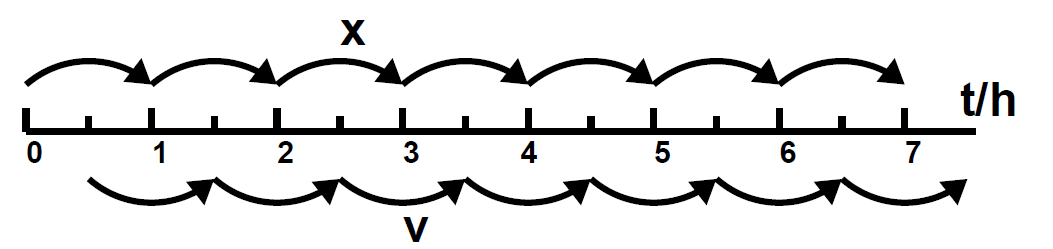
\includegraphics[width=0.5\textwidth]{Leapfrog}
  \caption{The Leapfrog integration principle, velocity and location are integrated in order rather than simultaneously}
  \label{fig:leapfrog}
\end{figure}
What makes Leapfrog preferable over Euler's method and Runge-Kutta 4, is that Leapfrog is stable for oscillary motion, under the conditon that \(dt<\frac{\pi R_i}{\tau_i}\), where \(R_i\) is the average radius of an orbit and \(\tau_i\) is the average orbital period\cite{LFcond}. 
The Leapfrog scheme used in this model is given below:
\begin{align*}
x_i
\end{align*}


\subsection{Collisions}
At certain times during the process, it may occur that the paths of two bodies intersect; a collision between bodies takes place. In order to numerically integrate the evolution of the system however, it is required to make a discretisation of time.
 Therefore, there is a non-trivial chance that a collision occurs in the system, which is overlooked due to the discretisation.
 In order to capture these moments, we note that a collision takes place during the \(n\)-th if at any given time \(t\in[t_{n},t_{n+1}]\), the distance \(d_{ij}(t)\) between the center of mass of each body is smaller then \(r_i+r_j\). 
 Here \(t_n=n\cdot dt\) (the start of the \(n\)-th month). This is illustrated in Figure \ref{fig:bots}.
 
\begin{figure}[H]
  \centering
  \includegraphics[width=0.5\textwidth]{botsingnaderbekeken}
  \caption{An illustration of intersecting paths of two celestial bodies}
  \label{fig:bots}
\end{figure}
 To formalise this principle, we linearise the path of \(i\) and \(j\) as follows: 
 Let \(\vec{x_i}\) be the location of body \(i\) at \(t=t_n\) and let \(\vec{v_i}\) be the numerically determined speed at \(t=t_{n+\frac{1}{2}}\).
The path of \(i\) is then given by:
\begin{align*}
\vec{\gamma_i}:[0,dt]\rightarrow\mathbb{R}^2 \\
t\mapsto \vec{x_i}+\vec{v_i}t
\end{align*}
And we can define the distance between \(i\) and \(j\) as:
\begin{align*}
	d_{ij}&:[0,dt]\rightarrow \mathbb{R}_{\geq 0}\\
	t&\mapsto \sqrt{(\vec{\gamma_i}(t)-\vec{\gamma_j}(t))\cdot(\vec{\gamma_i}(t)-\vec{\gamma_j}(t))}
\end{align*}
 A collision takes place in the \(n\)-th month if 
 \begin{align*}
	d_{ij}(t)^2&=(\vec{x_i}+\vec{v_i}t-(\vec{x_j}+\vec{v_j}t))\cdot (\vec{x_i}+\vec{v_i}t-(\vec{x_j}+\vec{v_j}t))\\
	&= (\Delta\vec{x} +t\Delta\vec{v})\cdot(\Delta\vec{x} +t\Delta\vec{v})<(r_i+r_j)^2
 \end{align*}
  The distance obtains its minimum when \(\frac{d}{dt}d_{ij}(t)^2=0\). Thus for \(t\) we find:
  \begin{align*}
  0&=\frac{d}{dt}d_{ij}(t)^2 =2\Delta\vec{v}\cdot(\Delta\vec{x}+t\Delta\vec{v})\\
  t&=-\frac{\Delta\vec{v}\cdot \Delta\vec{x}}{||\Delta \vec{v}||^2}
  \end{align*}
  Thus we can conclude, bodies \(i\) and \(j\) collide if:
 \begin{enumerate}
  \item \(0\leq t \leq \Delta t\) 
  \item \((\Delta\vec{x} +t\Delta\vec{v})\cdot(\Delta\vec{x} +t\Delta\vec{v}) <(r_i+r_j)^2\)
\end{enumerate} 
where \(t= -\frac{\Delta\vec{v}\cdot \Delta\vec{x}}{||\Delta \vec{v}||^2}\).\\
In this model, we assume that when two planets \(i\) and \(j\) collide, a new planet \(k\) is formed. When two planets collide, the planets will almost surely break into smaller fragments. 
Due to the gravitational forces however, these small fragements will be pulled back together and therefore our assumption that one new planet is formed is reasonable.
For this new planet, the mass, velocity and location are determined by the mass, velocity and location of the older planets. 
Due to the conservation of mass, we have \(m_k=m_j+m_i\). We set \(\vec{x_k}=\frac{1}{2}(\vec{x_i}+\vec{x_j})\). Due to the conservation of momentum, we can determine the new velocity: 
\begin{align*}
	m_k\vec{v_k}=m_j\vec{v_j}+m_i\vec{v_i}\\
	\vec{v_k}=\frac{1}{m_i+m_j}(m_j\vec{v_j}+m_i\vec{v_i})
\end{align*}
This process of creating new planets is the very foundation of the system and evolution of systems. With this properly defined, we are now able to simulate the evolution of planetary systems.
\subsection{Gaseous planets}
Thusfar we have assumed that every planet consists of just one (solid) material. 
In general however, this may not necessarily be the case, Jupiter for instance consists mostly of Hydrogen. Its solid core only makes up for only 25\% of its diameter.
This allows a modifcation of the model, in which every celestial body is not just made of rock, but consists of a solid core, with a gaseous atmosphere. 
In this model, we will classify the original in two different types: Solid bodies and gaseous bodies.
 Solid bodies consist for 100\% of rock, whereas gaseous bodies consist 90\% of hydrogen and 10\% of rock (in terms of mass). To implement this modification, we have to adjust certain definitions in our current system. Firstly, we have to modify our definition of the radius as given in Equation \eqref{eq:rad}. In the new model, Equation \eqref{eq:rad} reformulates itself to
 \begin{align*}
 r_i=\sqrt[3]{\frac{3 m_i^s}{4\pi \rho_s}+\frac{3 m_i^g}{4\pi \rho_g}}
 \end{align*}
 Here \(m_i^s\) is the mass of the solid core, and \(m_i^g\) the mass of the gaseous atmosphere. \(\rho_s\) is the mass density of the core and \(\rho_g\) is the mass density of the gaseous atmosphere. We assume that the solid core has the same density as the Earth and that the atmosphere has the same density as Saturn. Rescaling then gives us:
 \begin{align*}
 \rho_s =3.115\cdot 10^{12}{M_{\oplus}}/{\text{AU}^3} && \rho_g = 3.884\cdot 10^{11}{M_{\oplus}}/{\text{AU}^3}
 \end{align*}
